%-----------------------------------------------------------------
\section{Base Boards}
\label{sec:base}
%-----------------------------------------------------------------
The FLEX Base Boards are designed to export all the connections of a standard Microchip dsPIC� DSC micro-controller. The board connections use the standard 2.54mm pitch; this feature make it easy the usage of customised (by Evidence) or home-made Daughter Boards.\\

\noindent The dsPIC� DSC micro-controllers can be mounted on boards in two different ways:
\begin{enumerate}
  \item by soldering the micro-controller directly on the surface of the board, or
  \item by  using a socket for installing the micro-controller through the interchangeable Plug-In Modules (PIMs) available from Microchip.
\end{enumerate}
With the later, the developer need not worry about the number of programming cycles during the implementation/test/debugging phases, as once the limit is reached, a new PIM can be installed on the socket replacing the older one.\\

\begin{figure}[!ht]
	\centering
		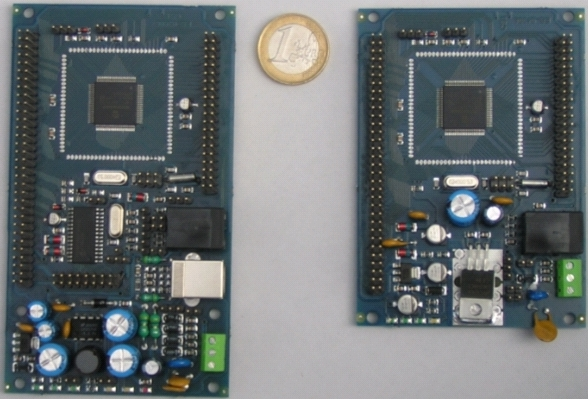
\includegraphics[width=0.90\textwidth,bb=0 0 588 399]{images/baseboards.jpg}
	\caption{FLEX Base Boards}
	\label{fig:base}
\end{figure}

\noindent As decipted in Figure ~\ref{fig:base}, The FLEX Base Board is available in two versions:
\begin{enumerate}
  \item Light version, refer Subsection ~\ref{subsec:001}
  \item Full version, refer Subsection ~\ref{subsec:003}
\end{enumerate}

\noindent The connectors of the Full and Light Versions are fully compatible, so that an application developed with the Full Version can be easily moved to the Light Version and vice-versa (i.e. with fewer or no modification to the control program).\\

\noindent Safety has been one of the most important aspect considered while engineering both versions of FLEX. Both the Base Boards are protected by a resettable fuse, permitting longer duration of the board, even when used by non-highly-skilled users (i.e. in school laboratories for students experiments).\\

\noindent Table ~\ref{tbl:base} compares FLEX Full with FLEX Light.
\begin{small}
\begin{table} [!ht]
\centering
\begin{tabular}{|p{0.8\columnwidth}|c|c|}
	\hline
	{\bf Features} & {\bf Full} & {\bf Light}\\
	\hline \hline
	Microchip dsPIC� DSC microcontroller dsPIC33FJ256MC710 & $\bullet$ & $\bullet$\\
  \hline
  Microchip PIC18� PIC18F2550 microcontroller for USB connection (programming using the USB port would be made available very soon) & $\bullet$ & \\
  \hline
  ICD2 in-circuit program connector & $\bullet$ & $\bullet$\\
  \hline
  USB connector for communication & $\bullet$ & \\
  \hline
  Set of LEDs for monitoring the board functioning status & $\bullet$ & $\bullet$\\
  \hline
  Set of connectors for Daughter boards piggybacking & $\bullet$ & $\bullet$\\
  \hline
  Power supply connectors & $\bullet$ & $\bullet$\\
  \hline
  Power supply circuitry with resettable fuses & $\bullet$ & $\bullet$\\
  \hline
  Simplified power supply (7 - 12V) & & $\bullet$\\
  \hline
  Extra-robust switching power supply (9 - 36V) & $\bullet$ & \\
  \hline
\end{tabular}
\caption{FLEX Full Vs FLEX Light}
\label{tbl:base}
\end{table}
\end{small}



%+-+-+-+-+-+-+-+-+-+-+-+-+-+-+-+-+-+-+-+-+-+-+-+-+-+-+-+-+-+-+-+-+
\clearpage
\subsection{[FLEX001] FLEX Light Base Board}
\label{subsec:001}
%+-+-+-+-+-+-+-+-+-+-+-+-+-+-+-+-+-+-+-+-+-+-+-+-+-+-+-+-+-+-+-+-+
The FLEX Light, as depicted in Figure ~\ref{fig:001}, has been designed to be as compact as possible. The Light Version uses a simplified power supply circuitry and there is no integrated USB programming capability. Target applications for the FLEX Light could be: distributed, battery-powered applications, like sensor networks; small robotic applications, i.e., for mobile robot control and sensor acquisition, etc.\\

\noindent The power supply of the FLEX Light varies in the range of 9 - 12V.\\

\begin{figure}[!ht]
	\centering
		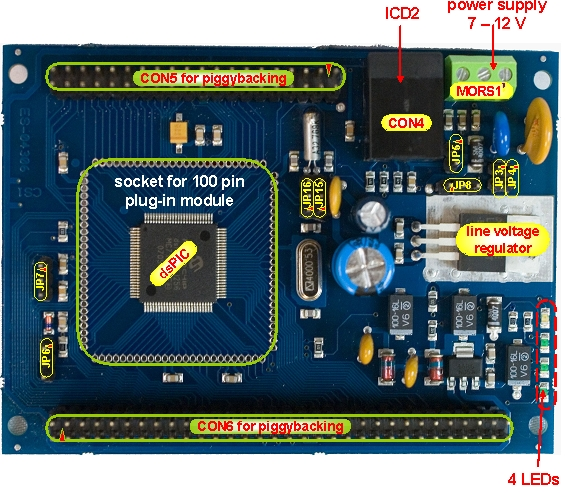
\includegraphics[width=0.90\textwidth,bb=0 0 582 493]{images/flex001.jpg}
	\caption{[FLEX001] FLEX Light Base Board}
	\label{fig:001}
\end{figure}

\noindent The main components of the FLEX Light are:
\begin {itemize}
  \item Microchip dsPIC� DSC microcontroller dsPIC33FJ256MC710
  \item A socket for the 100 pin Plug-In Module (PIM) available from Microchip
  \item An ICD2 programmer connector
  \item Power supply connectors
  \item A set of LEDs for monitoring the board functioning status
  \item Set of connectors for Daughter boards piggybacking
\end {itemize}


%^^^^^^^^^^^^^^^^^^^^^^^^^^^^^^^^^^^^^^^^^^^^^^^^^^
\subsubsection{Technical details}
\label{subsubsec:001tech}
%^^^^^^^^^^^^^^^^^^^^^^^^^^^^^^^^^^^^^^^^^^^^^^^^^^
\begin{figure}[!ht]
	\centering
		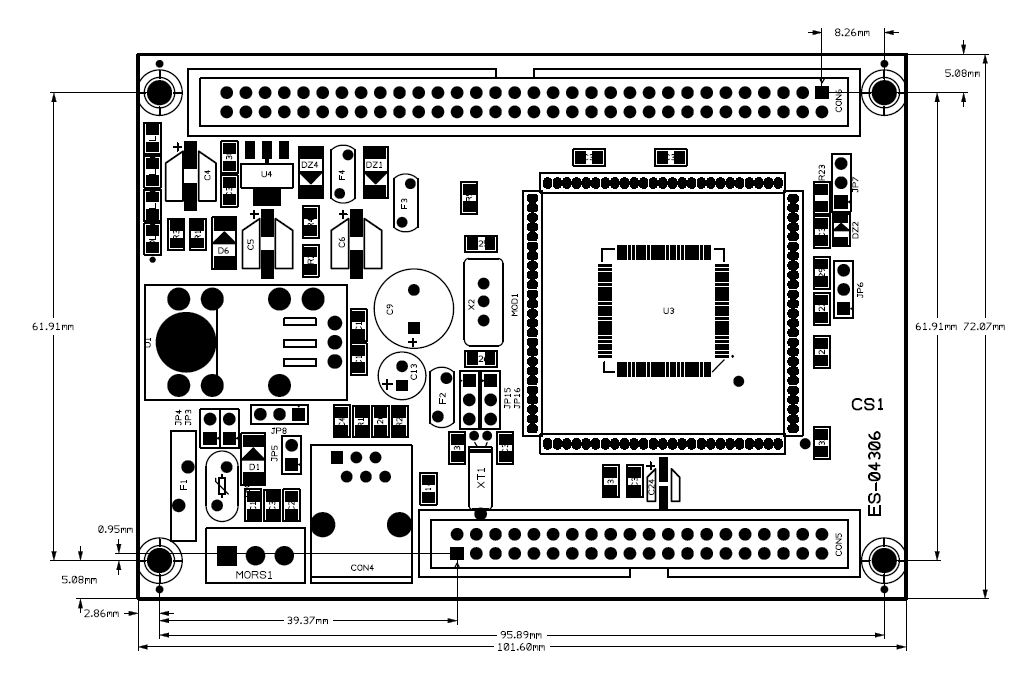
\includegraphics[width=0.90\textwidth,bb=0 0 1019 677]{images/001mec.png}
	\caption{[FLEX001] Dimensions of FLEX Light Base Board}
	\label{fig:001mec}
\end{figure}
\begin{figure}[!ht]
	\centering
		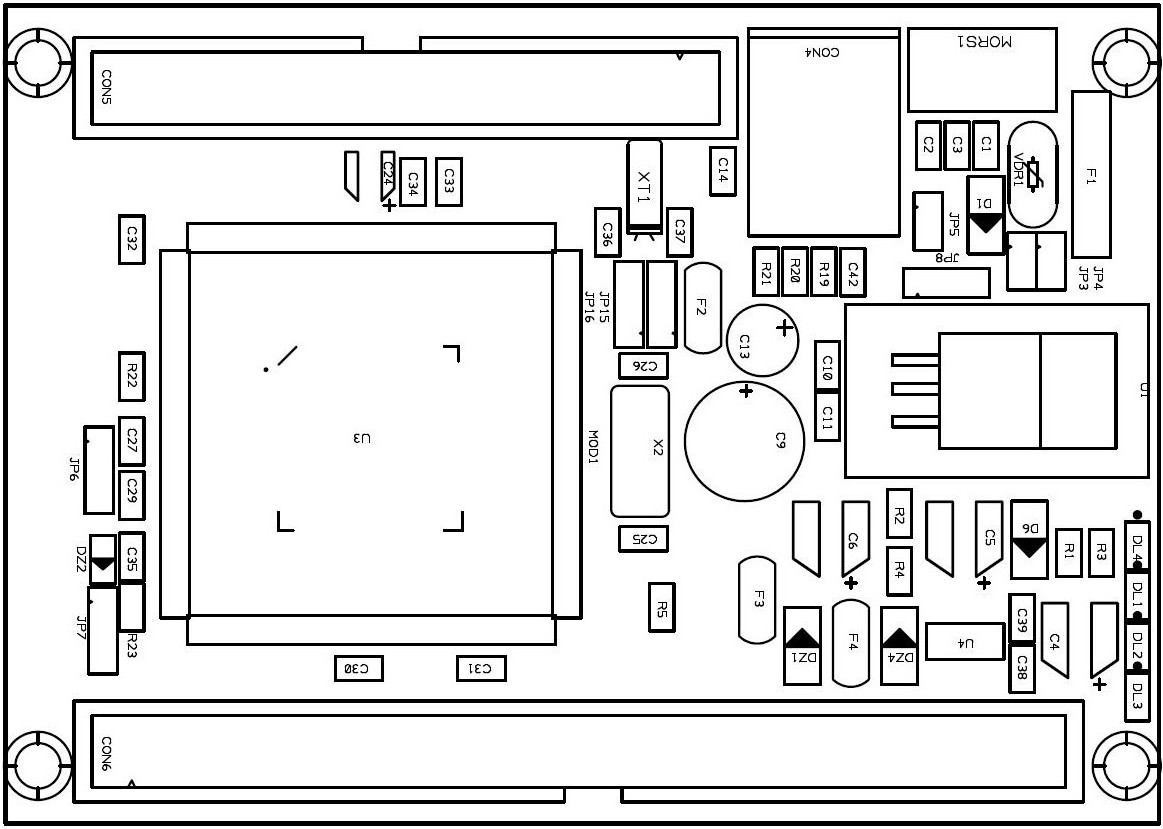
\includegraphics[width=0.90\textwidth,bb=0 0 1163 829]{images/001.png}
	\caption{[FLEX001] Details of FLEX Light Base Board}
	\label{fig:001detail}
\end{figure}


\begin{small}
\begin{table} [!ht]
\centering
\begin{tabular}{|c|l|}
  \hline
  Pin 1 & VIN\\
  \hline
  Pin 2 & GND\\
  \hline
  Pin 3 & EARTH\\
  \hline
\end{tabular}
\caption{FLEX001 - MORS1 (7-12 V power supply)}
\label{tbl:001mors1}
\end{table}
\end{small}


\begin{small}
\begin{table} [!ht]
\centering
\begin{tabular}{|l|l|}
  \hline
  DL1 (green) & Input power supply\\
  \hline
  DL2 (green) & Internal +5V power line activity\\
  \hline
  DL3 (green) & Internal +3V power line activity\\
  \hline
  DL4 (yellow) & dsPIC� DSC  (e.g. for debugging)\\
  \hline
\end{tabular}
\caption{FLEX001 - LEDs}
\label{tbl:001leds}
\end{table}
\end{small}


\begin{small}
\begin{table} [!ht]
\centering
\begin{tabular}{|c|c|c|}
  \hline
  {\bf Jumper} & {\bf pos. 1-2} & {\bf pos. 2-3}\\
  \hline
  JP3 & $\bullet$ GND & -\\
  \hline
  JP4 & $\bullet$ GND & -\\
  \hline
  JP5 & $\bullet$ EARTH & -\\
  \hline
  JP6 & $\bullet$ +3.3V & +AV DD$_{ext}$\\
  \hline
  JP7 & $\bullet$ GND & AV SS$_{ext}$\\
  \hline
  JP8 & +5V & $\bullet$ +3.3V\\
  \hline
  JP15 & SOSCI & $\bullet$ CRYSTAL\\
  \hline
  JP16 & SOSCO & $\bullet$ CRYSTAL\\
  \hline
  \multicolumn{3}{l}{\begin{tiny}Note: Default jumper settings are indicated by a $\bullet$\end{tiny}}\\
\end{tabular}
\caption{FLEX001 - Jumpers}
\label{tbl:001jps}
\end{table}
\end{small}


\begin{small}
\begin{table} [!ht]
\centering
\begin{tabular}{|l|l||l|l|}
  \hline
  Pin 1 & V$_{out}$ & Pin 2 & 5V$_{out}$\\
  \hline
  Pin 3 & Gnd$_{out}$ & Pin 4 & 3V$_{out}$\\
  \hline
  Pin 5 & INT3/RA14 & Pin 6 & GND\\
  \hline
  Pin 7 & IC1/RD8 & Pin 8 & INT4/RA15\\
  \hline
  Pin 9 & IC3/RD10 & Pin 10 & IC2/RD9\\
  \hline
  Pin 11 & OC1/RD0 & Pin 12 & IC4/RD11\\
  \hline
  Pin 13 & OC3/RD2 & Pin 14 & OC2/RD1\\
  \hline
  Pin 15 & IC5/RD12 & Pin 16 & OC4/RD3\\
  \hline
  Pin 17 & OC5/CN13/RD4 & Pin 18 & IC6/CN19/RD13\\
  \hline
  Pin 19 & OC7/CN15/RD6 & Pin 20 & OC6/CN14/RD5\\
  \hline
  Pin 21 & C1RX/RF0 & Pin 22 & OC8/UPDNCN16/RD7\\
  \hline
  Pin 23 & C2TX/RG1 & Pin 24 & C1TX/RF1\\
  \hline
  Pin 25 & AN22/CN22/RA6 & Pin 26 & C2RX/RG0\\
  \hline
  Pin 27 & PWM1L/RE0 & Pin 28 & AN23/CN23/RA7\\
  \hline
  Pin 29 & CSCK/RG14 & Pin 30 & PWM1H/RE1\\
  \hline
  Pin 31 & CSD0/RG13 & Pin 32 & CSDI/RG12\\
  \hline
  Pin 33 & PWM2H/RE3 & Pin 34 & PWM2L/RE2\\
  \hline
  Pin 35 & COFS/RG15 & Pin 36 & PWM3L/RE4\\
  \hline
  Pin 37 & PWM4L/RE6 & Pin 38 & PWM3H/RE5\\
  \hline
  Pin 39 & AN16/T2CK/T7CK/RC1 & Pin 40 & PWM4H/RE7\\
  \hline
\end{tabular}
\caption{FLEX001/FLEX003 - CON5 for Piggybacking}
\label{tbl:con5}
\end{table}
\end{small}


\begin{small}
\begin{table} [!ht]
\centering
\begin{tabular}{|l|l||l|l|}
  \hline
  Pin 1 & GND & Pin 2 & GND\\
  \hline
  Pin 3 & GND & Pin 4 & GND\\
  \hline
  Pin 5 & \begin{tiny}PGD2/EMUD2/SOSCI/CN1/RC13\end{tiny} & Pin 6 & \begin{tiny}PGC2/EMUC2/SOSCO/T1CK/CN0/RC14\end{tiny}\\
  \hline
  Pin 7 & AN17/T3CK/T6CK/RC2 & Pin 8 & AN18/T4CK/T9CK/RC3\\
  \hline
  Pin 9 & AN19/T5CK/T8CK/RC4 & Pin 10 & SCK2/CN8/RG6\\
  \hline
  Pin 11 & SDI2/CN9/RG7 & Pin 12 & SDO2/CN10/RG8\\
  \hline
  Pin 13 & DSP$_{MCLR}$ & Pin 14 & SS2/CN11/RG9\\
  \hline
  Pin 15 & TMS/RA0 & Pin 16 & AN20/FLTA/INT1/RE8\\
  \hline
  Pin 17 & AN21/FLTB/INT2/RE9 & Pin 18 & AN5/QEB/CN7/CN7/RB5\\
  \hline
  Pin 19 & AN4/QEA/CN6/RB4 & Pin 20 & AN3/INDX/CN5/RB3\\
  \hline
  Pin 21 & AN2/SS1/CN4/RB2 & Pin 22 & V$_{ref-}$/RA9\\
  \hline
  Pin 23 & V$_{ref+}$/RA10 & Pin 24 & AV DD$_{ext}$\\
  \hline
  Pin 25 & AV SS$_{ext}$ & Pin 26 & AN8/RB8\\
  \hline
  Pin 27 & AN9/RB9 & Pin 28 & AN10/RB10\\
  \hline
  Pin 29 & AN11/RB11 & Pin 30 & TCK/RA1\\
  \hline
  Pin 31 & U2CTS/RF12 & Pin 32 & U2RTS/RF13\\
  \hline
  Pin 33 & AN13/RB13 & Pin 34 & AN12/RB12\\
  \hline
  Pin 35 & IC7/U1CTS/CN20/RD14 & Pin 36 & AN15/OCFB/CN12/RB15\\
  \hline
  Pin 37 & U2RX/CN17/RF4 & Pin 38 & IC8/U1RTS/CN21/RD15\\
  \hline
  Pin 39 & U1TX/RF3 & Pin 40 & U2TX/CN18/RF5\\
  \hline
  Pin 41 & SDO1/RF8 & Pin 42 & U1RX/RF2\\
  \hline
  Pin 43 & SCK1/INT0/RF6 & Pin 44 & SDI1/RF7\\
  \hline
  Pin 45 & SCL1/RG2 & Pin 46 & SDA1/RG3\\
  \hline
  Pin 47 & SDA2/RA3 & Pin 48 & SCL2/RA2\\
  \hline
  Pin 49 & TD0/RA5 & Pin 50 & TDI/RA4\\
  \hline
  Pin 51 & PGD3/EMUD3/AN0/CN2/RB0 & Pin 52 & DSP$_{PCLK}$\\
  \hline
  Pin 53 & PGC3/EMUC3/AN1/CN3/RB1 & Pin 54 & DSP$_{PDATA}$\\
  \hline
  Pin 55 & 5V$_{out}$ & Pin 56 & 5V$_{out}$\\
  \hline
  Pin 57 & 3V$_{out}$ & Pin 58 & 3V$_{out}$\\
  \hline
  Pin 59 & GND & Pin 60 & GND\\
  \hline
  Pin 61 & V$_{out}$ & Pin 62 & V$_{out}$\\
  \hline
  Pin 63 & GND$_{out}$ & Pin 64 & GND$_{out}$\\
  \hline
\end{tabular}
\caption{FLEX001/FLEX003 - CON6 for Piggybacking}
\label{tbl:con6}
\end{table}
\end{small}



\begin{small}
\begin{table} [!ht]
\centering
\begin{tabular}{|l|}
  \hline
  $\bullet$ \hspace{0.1cm} {\tt CON4:} ICD2 connector\\
  \hline
\end{tabular}
\caption{FLEX001 - Other Connectors}
\label{tbl:001other}
\end{table}
\end{small}





%+-+-+-+-+-+-+-+-+-+-+-+-+-+-+-+-+-+-+-+-+-+-+-+-+-+-+-+-+-+-+-+-+
\clearpage
\subsection{[FLEX003] FLEX Full Base Board}
\label{subsec:003}
%+-+-+-+-+-+-+-+-+-+-+-+-+-+-+-+-+-+-+-+-+-+-+-+-+-+-+-+-+-+-+-+-+
The FLEX Full, as depicted in Figure ~\ref{fig:003}, integrates an extra-robust power supply circuitry, that allows usage of a wide range of power suppliers. It accepts voltage ranges between 9 - 36 volts. The power supply signal is filtered and adapted to the internal levels.\\
\begin{figure}[!ht]
	\centering
		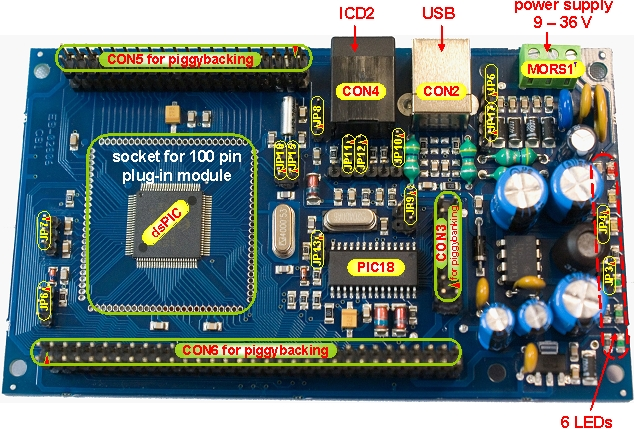
\includegraphics[width=0.90\textwidth,bb=0 0 635 436]{images/flex003.jpg}
	\caption{[FLEX003] FLEX Full Base Board}
	\label{fig:003}
\end{figure}

\noindent The FLEX Full also includes a native USB port which can be used for data transfer and, much more importantly as a programming interface for the onboard dsPIC� DSC. This option allows to save the cost of the ICD2 programming device, thereby making the development board fully self-contained.\\

\noindent {\tt Please note that the programming and debugging functionality on the PIC18 is not yet available. An application note will be available soon with all the needed information on how to implement the programmer functionality on the PIC18. The debugger functionality will be available as special version of the FLEX Full.}\\
 
\noindent The main components of FLEX Full are: 
\begin {itemize}
  \item Microchip dsPIC� DSC microcontroller dsPIC33FJ256MC710
  \item A socket for the 100 pin Plug-In Module (PIM) available from Microchip
  \item An ICD2 programmer connector
  \item A USB connector for direct programming
  \item Power supply connectors
  \item A set of LEDs for monitoring the board functioning status
  \item An onboard Microchip PIC18� PIC18F2550 microcontroller for integrated programming
  \item Set of connectors for Daughter boards piggybacking
\end {itemize}


%^^^^^^^^^^^^^^^^^^^^^^^^^^^^^^^^^^^^^^^^^^^^^^^^^^
\subsubsection{Technical details}
\label{subsubsec:003tech}
%^^^^^^^^^^^^^^^^^^^^^^^^^^^^^^^^^^^^^^^^^^^^^^^^^^
\begin{figure}[!ht]
	\centering
		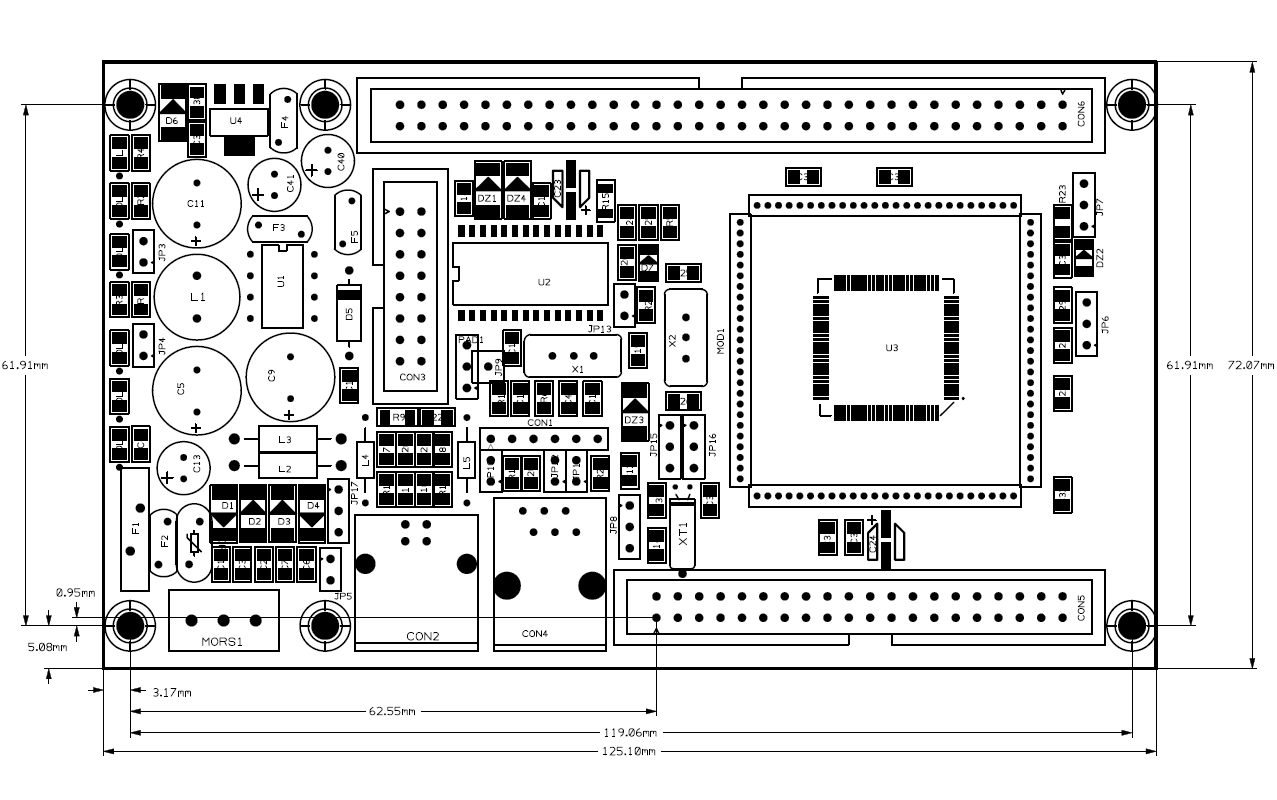
\includegraphics[width=0.90\textwidth,bb=0 0 1277 800]{images/003mec.png}
	\caption{[FLEX003] Dimensions of FLEX Full Base Board}
	\label{fig:003mec}
\end{figure}
\begin{figure}[!ht]
	\centering
		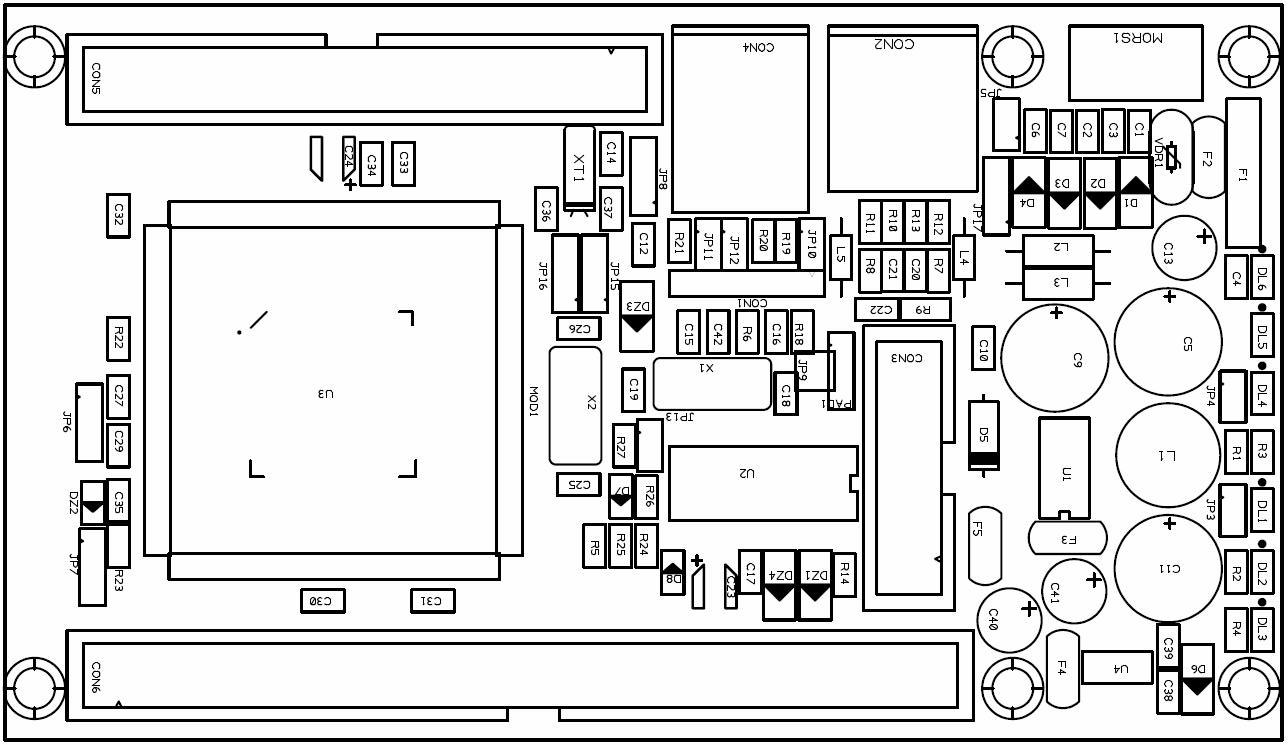
\includegraphics[width=0.90\textwidth,bb=0 0 1288 745]{images/003.png}
	\caption{[FLEX003] Details of FLEX Full Base Board}
	\label{fig:003detail}
\end{figure}

\begin{small}
\begin{table} [!ht]
\centering
\begin{tabular}{|c|l|}
  \hline
  Pin 1 & VINA\\
  \hline
  Pin 2 & VINB\\
  \hline
  Pin 3 & EARTH\\
  \hline
\end{tabular}
\caption{FLEX003 - MORS1 (9-36 V power supply)}
\label{tbl:003mors1}
\end{table}
\end{small}


\begin{small}
\begin{table} [!ht]
\centering
\begin{tabular}{|l|l|}
  \hline
  DL1 (green) & Input power supply\\
  \hline
  DL2 (green) & Internal +5V power line activity\\
  \hline
  DL3 (green) & Internal +3V power line activity\\
  \hline
  DL4 (yellow) & dsPIC� DSC  (e.g. for debugging)\\
  \hline
  DL5 (yellow) & Internal PIC18\\
  \hline
  DL6 (red) & USB cable connection monitor\\
  \hline
\end{tabular}
\caption{FLEX003 - LEDs}
\label{tbl:003leds}
\end{table}
\end{small}


\begin{small}
\begin{table} [!ht]
\centering
\begin{tabular}{|c|c|c|}
  \hline
  {\bf Jumper} & {\bf pos. 1-2} & {\bf pos. 2-3}\\
  \hline
  JP3 & $\bullet$ GND & -\\
  \hline
  JP4 & $\bullet$ GND & -\\
  \hline
  JP5 & $\bullet$ EARTH & -\\
  \hline
  JP6 & $\bullet$ +3.3V & +AV DD$_{ext}$\\
  \hline
  JP7 & $\bullet$ GND & AV SS$_{ext}$\\
  \hline
  JP8 & +5V & $\bullet$ +3.3V\\
  \hline
  JP9 & +USB & $\bullet$ +5V\\
  \hline
  JP10 & $\bullet$ DSP\_MCLR & PIC18\_MCLR\\
  \hline
  JP11 & $\bullet$ DSP\_PDATA & PIC18\_PDATA\\
  \hline
  JP12 & $\bullet$ DSP\_PCLK & PIC18\_PCLK\\
  \hline
  JP13 & VDD pull up & -\\
  \hline
  JP15 & SOSCI & $\bullet$ CRYSTAL\\
  \hline
  JP16 & SOSCO & $\bullet$ CRYSTAL\\
  \hline
  JP17 & $\bullet$ GND & EARTH\\
  \hline
  \multicolumn{3}{l}{\begin{tiny}Note: Default jumper settings are indicated by a $\bullet$\end{tiny}}\\
\end{tabular}
\caption{FLEX003 - Jumpers}
\label{tbl:003jps}
\end{table}
\end{small}


\begin{small}
\begin{table} [!ht]
\centering
\begin{tabular}{|l|l||l|l|}
  \hline
  Pin 1 & +VDD$_{out}$ & Pin 2 & GND\\
  \hline
  Pin 3 & RA0/AN0 & Pin 4 & RB4/AN11/KB10\\
  \hline
  Pin 5 & RA1/AN1 & Pin 6 & RB3/AN9/CCP2/VPO\\
  \hline
  Pin 7 & RA2/AN2/V$_{ref-}$/CV$_{ref}$ & Pin 8 & RC7/RX/DT/SDO\\
  \hline
  Pin 9 & RA3/AN3/Vref+ & Pin 10 & RC6/TX/CK\\
  \hline
  Pin 11 & RA5/AN4/HLVDin/C2$_{out}$ & Pin 12 & RC2/CCP1\\
  \hline
  Pin 13 & RC1/T1OSI/CCP2/UOE\# & Pin 14 & RA4/T0CKI/C1$_{out}$/RCV\\
  \hline
  Pin 15 & L$_{MCLR}$ & Pin 16 & RC0/T1OSO/T1CKI\\
  \hline
\end{tabular}
\caption{FLEX003 - CON3 for Piggybacking (PIC18F2550)}
\label{tbl:con3}
\end{table}
\end{small}


\begin{small}
\begin{table} [!ht]
\centering
\begin{tabular}{|l|}
  \hline
  $\bullet$ \hspace{0.1cm} {\tt CON2:} USB connector\\
  $\bullet$ \hspace{0.1cm} {\tt CON4:} ICD2 connector\\
  $\bullet$ \hspace{0.1cm} {\tt CON5:} 40 pin piggybacking connector, refer Table \ref{tbl:con5} \\
  $\bullet$ \hspace{0.1cm} {\tt CON6:} 64 pin piggybacking connector, refer Table \ref{tbl:con6} \\
  \hline
\end{tabular}
\caption{FLEX003 - Other Connectors}
\label{tbl:003other}
\end{table}
\end{small}


\begin{small}
\begin{table} [!ht]
\centering
\begin{tabular}{|c|c|c|}
  \hline
  {\bf Jumper} & {\bf pos. 1-2} & {\bf pos. 2-3}\\
  \hline
  JP3 & $\bullet$ & -\\
  \hline
  JP4 & $\bullet$ & -\\
  \hline
  JP5 & $\bullet$ & -\\
  \hline
  JP6 & $\bullet$ & \\
  \hline
  JP7 & $\bullet$ & \\
  \hline
  JP8 & $\bullet$ & \\
  \hline
  JP9 &  & $\bullet$\\
  \hline
  JP10 &  & $\bullet$\\
  \hline
  JP11 &  & $\bullet$\\
  \hline
  JP12 &  & $\bullet$\\
  \hline
  JP13 &  & -\\
  \hline
  JP15 &  & $\bullet$\\
  \hline
  JP16 &  & $\bullet$\\
  \hline
  JP17 & $\bullet$ & \\
  \hline
\end{tabular}
\caption{FLEX003 - Jumper settings for programming PIC18}
\label{tbl:003pic18}
\end{table}
\end{small}